\documentclass{beamer}
\usepackage{amsmath}
\usepackage{hyperref}
\usepackage{listings}
\usepackage{xcolor}
\hypersetup{colorlinks=true, citecolor=blue, filecolor=blue, linkcolor=blue, urlcolor=blue}
\definecolor{codegreen}{rgb}{0,0.6,0}
\definecolor{codegray}{rgb}{0.5,0.5,0.5}
\definecolor{codepurple}{rgb}{0.58,0,0.82}
\definecolor{backcolour}{rgb}{0.95,0.95,0.92}
 
\lstdefinestyle{mystyle}{
    backgroundcolor=\color{backcolour},   
    commentstyle=\color{codegreen},
    keywordstyle=\color{magenta},
    numberstyle=\tiny\color{codegray},
    stringstyle=\color{codepurple},
    basicstyle=\ttfamily\footnotesize,
    breakatwhitespace=false,         
    breaklines=true,                 
    captionpos=b,                    
    keepspaces=true,                 
    %numbers=left,                    
    numbersep=5pt,                  
    showspaces=false,                
    showstringspaces=false,
    showtabs=false,                  
    tabsize=2
}
 
\lstset{style=mystyle}

\mode<presentation> {

% The Beamer class comes with a number of default slide themes
% which change the colors and layouts of slides. Below this is a list
% of all the themes, uncomment each in turn to see what they look like.

%\usetheme{default}
\usetheme{AnnArbor}
%\usetheme{Antibes}
%\usetheme{Bergen}
%\usetheme{Berkeley}
%\usetheme{Berlin}
%\usetheme{Boadilla}
%\usetheme{CambridgeUS}
%\usetheme{Copenhagen}
%\usetheme{Darmstadt}
%\usetheme{Dresden}
%\usetheme{Frankfurt}
%\usetheme{Goettingen}
%\usetheme{Hannover}
%\usetheme{Ilmenau}
%\usetheme{JuanLesPins}
%\usetheme{Luebeck}
%\usetheme{Madrid}
%\usetheme{Malmoe}
%\usetheme{Marburg}
%\usetheme{Montpellier}
%\usetheme{PaloAlto}
%\usetheme{Pittsburgh}
%\usetheme{Rochester}
%\usetheme{Singapore}
%\usetheme{Szeged}
%\usetheme{Warsaw}

% As well as themes, the Beamer class has a number of color themes
% for any slide theme. Uncomment each of these in turn to see how it
% changes the colors of your current slide theme.

%\usecolortheme{albatross}
%\usecolortheme{beaver}
%\usecolortheme{beetle}
%\usecolortheme{crane}
%\usecolortheme{dolphin}
%\usecolortheme{dove}
%\usecolortheme{fly}
%\usecolortheme{lily}
%\usecolortheme{orchid}
%\usecolortheme{rose}
%\usecolortheme{seagull}
%\usecolortheme{seahorse}
%\usecolortheme{whale}
%\usecolortheme{wolverine}

%\setbeamertemplate{footline} % To remove the footer line in all slides uncomment this line
\setbeamertemplate{footline}[page number] % To replace the footer line in all slides with a simple slide count uncomment this line

\setbeamertemplate{navigation symbols}{} % To remove the navigation symbols from the bottom of all slides uncomment this line
}

\usepackage{graphicx} % Allows including images
\usepackage{booktabs} % Allows the use of \toprule, \midrule and \bottomrule in tables
%\usepackage {tikz}
\usepackage{tkz-graph}
\GraphInit[vstyle = Shade]
\tikzset{
  LabelStyle/.style = { rectangle, rounded corners, draw,
                        minimum width = 2em, fill = yellow!50,
                        text = red, font = \bfseries },
  VertexStyle/.append style = { inner sep=5pt,
                                font = \normalsize\bfseries},
  EdgeStyle/.append style = {->, bend left} }
\usetikzlibrary {positioning}
%\usepackage {xcolor}
\definecolor {processblue}{cmyk}{0.96,0,0,0}
%----------------------------------------------------------------------------------------
%	TITLE PAGE
%----------------------------------------------------------------------------------------

\title[Gradient Descent]{Numerical Optimization 07: 2nd order methods} %

\author{Qiang Zhu} % Your name
\institute[University of Nevada Las Vegas] % Your institution as it will appear on the bottom of every slide, may be shorthand to save space
{
University of Nevada Las Vegas\\ % Your institution for the title page
\medskip
}
\date{\today} % Date, can be changed to a custom date

\begin{document}

\begin{frame}
\titlepage % Print the title page as the first slide
\end{frame}

\begin{frame}
\frametitle{Overview} % Table of contents slide, comment this block out to remove it
\tableofcontents % Throughout your presentation, if you choose to use \section{} and \subsection{} commands, these will automatically be printed on this slide as an overview of your presentation
\end{frame}

%----------------------------------------------------------------------------------------
%	PRESENTATION SLIDES
%----------------------------------------------------------------------------------------

%------------------------------------------------

\section{Newton's method}
\begin{frame}{Newton's method}
In optimization, knowing the first-order information can help determine the direction to travel, but does not help to determine how far to step to the local minimum. A better way is to use the second-order information.

In univariable optimization, the quadratic approximation about a point ($x^k$) come from 
\begin{equation*}
    q(x) = f(x^k) + (x-x^k)f`(x^k) + \frac{(x-x^k)^2}{2}f``(x^k)
\end{equation*} 
Setting the derivative to zero, 
\begin{equation*}
\begin{split}
		\frac{\partial q(x)}{\partial x} &= f`(x^k) + (x-x^k)f``(x^k) = 0 \\
		x^{k+1} &= x^k - \frac{f`(x^k)}{f``(x^k)}
\end{split}
\end{equation*}

\end{frame}

\begin{frame}{Various cases}
\begin{figure}
\centering
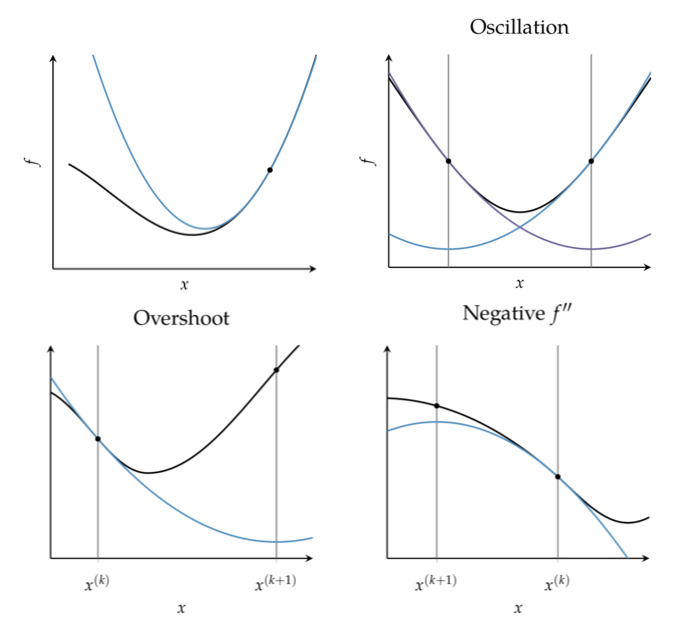
\includegraphics[width=80mm]{Figs/newton-1d.jpeg}
\end{figure}    
    
\end{frame}


\section{Extension to multivariate optimization}
\begin{frame}{Extension to multivariate optimization}
If $f$ is a multivariate function
\begin{equation*}
    f(\boldsymbol{x}) = f(\boldsymbol{x}^k) + (\boldsymbol{g}^k)^T(\boldsymbol{x}-\boldsymbol{x}^k) 
    + \frac{1}{2} (\boldsymbol{x}-\boldsymbol{x^k})^T \boldsymbol{H}^k (\boldsymbol{x}-\boldsymbol{x}^k) 
\end{equation*}

Setting the gradient to be zero,
\begin{equation*}
    \nabla q(\boldsymbol{x}^k) = \boldsymbol{g}^k + \boldsymbol{H}^k (\boldsymbol{x}-\boldsymbol{x}^k)
\end{equation*}

\begin{alertblock}{Quiz}
The Booth's function is
\begin{equation*}
    f(\boldsymbol{x}) = (x_1 + 2x_2 -7)^2 + (2x_1 + x_2 -5)^2
\end{equation*}
use the Newton's method to find the minimum when $\boldsymbol{x}$ =[9, 8]


\end{alertblock}

\end{frame}

\begin{frame}{Newton's method with line search}
Newton’s method can also be used to supply a descent direction to line search or can be modified to use a step factor. Smaller steps toward the minimum or line searches along the descent direction can increase the method’s robustness. The descent direction is:
    \begin{equation*}
        \boldsymbol{d}^k = -(\boldsymbol{H}^k)^{-1}\boldsymbol{g}^k
    \end{equation*}

\end{frame}

\section{Secant Method}
\begin{frame}{Secant Method}
Newton's method for \textcolor{blue}{univariate} function minimization needs to know the first and second derivatives. However, the second derivative is not easy to compute for some cases. The secant method use estimates of $H$ as follows
\begin{gather*}
    f``(x^k) \approx \frac{f`(x^k - f`(x^{k-1})} {x^k-x^{k-1}}
\end{gather*}

The secant method requires \textcolor{blue}{an additional initial design point}. It suffers from the same problems as Newton's method when quadratic function is not a good approximation.

\end{frame}



\section{Summary}
\begin{frame}{Summary}
    \begin{itemize}
        \item Incorporating second-order information in descent methods often speeds convergence.
        \item Newton’s method is a root-finding method that leverages second-order information to quickly descend to a local minimum.
        \item The secant method approximate Newton’s method when the second-order information is not directly available.
    \end{itemize}
\end{frame}
\end{document}

